\documentclass{article}
\usepackage{amsmath, amssymb, tikz, multicol, tcolorbox, array, sfmath, enumerate, pgfplots}
\renewcommand{\familydefault}{\sfdefault}
\pgfplotsset{compat=newest}
\usetikzlibrary{arrows.meta}
\everymath{\displaystyle}
\tikzset{>=stealth}
\tikzstyle{input} = [circle, text centered, radius = 1cm, draw = black]
\tikzstyle{function} = [rectangle, text centered, minimum width = 2cm, minimum height = 1cm, draw = black]
\usepackage[top = 0.25in, bottom = 0.25in, left = 1in, right = 1in]{geometry}
\pagestyle{empty}
\raggedright

\newcounter{example}[section]
\newenvironment{example}[1][]{\refstepcounter{example}\par\medskip
   {\color{red}\textbf{Example~\theexample. #1}}}{\medskip}

\begin{document}

\section*{Solving Equations and Inequalities}

\begin{tcolorbox}[colframe=orange!70!white, coltitle=black, title=\textbf{Summary}]
\begin{enumerate}
    \item Use reverse order of operations to solve equations.
    \item You can check your solutions numerically (plug the value of the variable into the original equation) or visually (find the $x$-coordinates of the intersection points).
    \item When solving inequalities, flip the inequality sign if you multiply or divide \underline{both} sides by a negative number.
\end{enumerate}
\end{tcolorbox}
\bigskip 

When solving an equation, our goal is to get the variable, usually $x$, alone on one side of the equal sign.	
\bigskip 

To do this, we use \textbf{reverse order of operations}:	
\begin{enumerate}
	\item Undo any addition or subtraction. 
	\item Undo any multiplication or division.
	\item Undo any exponents.
	\item Get rid of parentheses.
\end{enumerate}
\bigskip 

You can make sure your answer is correct by {\color{blue}\textbf{plugging it in}} to the original problem and seeing if the left side and right side are equal. 
\bigskip 

\begin{example}
Solve each of the following. Round to 2 decimal places when necessary.
\begin{enumerate}[(a)]
\begin{multicols}{3}
    \item $3x + 4 = 16$
    \item $-2x-9=17-x$
    \item $\frac{1}{2}x + 3 = \frac{2}{5}x$
\end{multicols}
\vfill 
\begin{multicols}{3}
    \item $2.1x - 7 = 23.83$
    \item $2(x-10) = 4(x-5)-2x$
    \item $3(x+4)+3x = 2(3x+5)-2$
\end{multicols}
\end{enumerate}
\vfill 
\end{example}

\newpage 


% Another useful way to help check your answers is to {\color{blue}\textbf{graph}} the left side of the equation, as well as the right side. \vspace{0.5in}

% The solution is the $x$-coordinate of their \textbf{intersection point}.	\vfill 

% For ``no solution'' answers ($\varnothing$), the graphs will \textbf{never intersect}. \vspace{0.25in}	

% For ``all real numbers'' answers ($\mathbb{R}$), the graphs will be \textbf{one in the same}. \vfill 

% \subsubsection*{Visual Way to Check Solutions}
% The graphs of $y = 3x+4$ and $y=16$ are shown below:	\newline\\
% \begin{center}
% \begin{tikzpicture}[scale=0.8]
%     \begin{axis}
%     [
%     xlabel = $x$,
%     ylabel = $y$,
%     axis lines = middle,
%     axis line style={stealth-stealth},
%     axis line style={shorten >=-7.5pt, shorten <=-7.5pt},
%     xmin = 0, xmax = 5,
%     ymin = 0, ymax = 20,
%     ystep = 4,
%     xtick = {-4,-3,...,4},
%     ytick = {4,8,...,20},
%     grid,
%     every axis x label/.style = {at = {(ticklabel* cs:1)}, anchor = south},
%     every axis y label/.style = {at = {(ticklabel* cs:1)}, anchor = west}
%     ]
%     \addplot[domain = 0:4.5, samples = 200, line width = 1.5, smooth, color=blue]{3*x+4};
%     \addplot[domain = 0:5, samples = 200, line width = 1.5, smooth, color=red] {16};
%     \addplot [mark = *] coordinates {(4, 16)} node [below right] {\textbf{(4, 16)}};
%     \end{axis}
%     \end{tikzpicture}
% \end{center}

\newpage 

\subsection*{Inequalities}

{\color{blue}\textbf{Inequalities typically give you an infinite number of solutions.}}	\newline

For instance, there are an infinite number of values that you can substitute into $x$ for $x > -4$ to make it true. 
\newline 

Since we can't list every possible solution, we can shade a region on a number line to represent this solution.	\newline\\	
\begin{center}
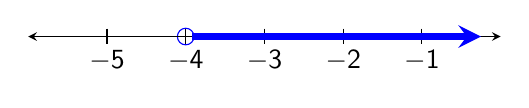
\begin{tikzpicture}
    \draw [color = blue] (-4,0) circle (3pt);
	\draw [<->, > = stealth] (-6,0) -- (-0,0);
	\foreach \x in {-5,-4,-3,-2,-1}
	\draw (\x, 0.1) -- (\x, -0.1);
	\foreach \x in {-5,-4,-3,-2,-1}
	\node at (\x, -0.3) {$\x$};
	\draw [->, color = blue, line width = 2.5, >=stealth] (-3.92,0) -- (-0.25,0);
\end{tikzpicture}
\end{center}
\bigskip 

\textsc{Summary of Graphing Inequalities}   \newline\\
If your variable is on the \textbf{left side} when graphing an inequality, you can use the following table to help you graph:	\newline\\
\begin{center}
\setlength{\extrarowheight}{4pt}
\begin{tabular}{c|c|c}  
\textbf{Expression}	&	\textbf{Circle}	&	\textbf{Shade}	\\
\hline
$x<$					&	Open				& 	Left		\\[4pt]
\hline
$x>$					&	Open				&	Right	\\[4pt]
\hline
$x \leq$				&	Closed			&	Left		\\[4pt]
\hline
$x \geq$				&	Closed			&	Right	\\[4pt]
\end{tabular}
\end{center}
\bigskip 

With solving inequalities, you must remember to flip the inequality sign if you multiply or divide {\color{blue}\textbf{both sides}} by a {\color{orange}\textbf{negative number}}.   \bigskip 

\begin{example}
Solve and graph each.
\begin{multicols}{2}
\begin{enumerate}[(a)]
    \item $3x - 5 > -17$    
    \item $-4x + 10 \leq 38$
\end{enumerate}
\end{multicols}

\vfill 

\begin{multicols}{2}
\begin{enumerate}[(a)]  \setcounter{enumi}{2}
    \item $2(x+4)-5 > 2x + 3$    
    \item $3(x+1) \geq 3x + 2$  
\end{enumerate}
\end{multicols}
\end{example}

\vfill 



\end{document}
